% Options for packages loaded elsewhere
\PassOptionsToPackage{unicode}{hyperref}
\PassOptionsToPackage{hyphens}{url}
%
\documentclass[
]{book}
\title{Mappeeksamen}
\usepackage{etoolbox}
\makeatletter
\providecommand{\subtitle}[1]{% add subtitle to \maketitle
  \apptocmd{\@title}{\par {\large #1 \par}}{}{}
}
\makeatother
\subtitle{\url{https://github.com/Margitsor/IDR4000-bookdown.git}}
\author{Margit Dahl Sørensen, Kandidatnummer:110}
\date{2021-12-02}

\usepackage{amsmath,amssymb}
\usepackage{lmodern}
\usepackage{iftex}
\ifPDFTeX
  \usepackage[T1]{fontenc}
  \usepackage[utf8]{inputenc}
  \usepackage{textcomp} % provide euro and other symbols
\else % if luatex or xetex
  \usepackage{unicode-math}
  \defaultfontfeatures{Scale=MatchLowercase}
  \defaultfontfeatures[\rmfamily]{Ligatures=TeX,Scale=1}
\fi
% Use upquote if available, for straight quotes in verbatim environments
\IfFileExists{upquote.sty}{\usepackage{upquote}}{}
\IfFileExists{microtype.sty}{% use microtype if available
  \usepackage[]{microtype}
  \UseMicrotypeSet[protrusion]{basicmath} % disable protrusion for tt fonts
}{}
\makeatletter
\@ifundefined{KOMAClassName}{% if non-KOMA class
  \IfFileExists{parskip.sty}{%
    \usepackage{parskip}
  }{% else
    \setlength{\parindent}{0pt}
    \setlength{\parskip}{6pt plus 2pt minus 1pt}}
}{% if KOMA class
  \KOMAoptions{parskip=half}}
\makeatother
\usepackage{xcolor}
\IfFileExists{xurl.sty}{\usepackage{xurl}}{} % add URL line breaks if available
\IfFileExists{bookmark.sty}{\usepackage{bookmark}}{\usepackage{hyperref}}
\hypersetup{
  pdftitle={Mappeeksamen},
  pdfauthor={Margit Dahl Sørensen, Kandidatnummer:110},
  hidelinks,
  pdfcreator={LaTeX via pandoc}}
\urlstyle{same} % disable monospaced font for URLs
\usepackage{longtable,booktabs,array}
\usepackage{calc} % for calculating minipage widths
% Correct order of tables after \paragraph or \subparagraph
\usepackage{etoolbox}
\makeatletter
\patchcmd\longtable{\par}{\if@noskipsec\mbox{}\fi\par}{}{}
\makeatother
% Allow footnotes in longtable head/foot
\IfFileExists{footnotehyper.sty}{\usepackage{footnotehyper}}{\usepackage{footnote}}
\makesavenoteenv{longtable}
\usepackage{graphicx}
\makeatletter
\def\maxwidth{\ifdim\Gin@nat@width>\linewidth\linewidth\else\Gin@nat@width\fi}
\def\maxheight{\ifdim\Gin@nat@height>\textheight\textheight\else\Gin@nat@height\fi}
\makeatother
% Scale images if necessary, so that they will not overflow the page
% margins by default, and it is still possible to overwrite the defaults
% using explicit options in \includegraphics[width, height, ...]{}
\setkeys{Gin}{width=\maxwidth,height=\maxheight,keepaspectratio}
% Set default figure placement to htbp
\makeatletter
\def\fps@figure{htbp}
\makeatother
\setlength{\emergencystretch}{3em} % prevent overfull lines
\providecommand{\tightlist}{%
  \setlength{\itemsep}{0pt}\setlength{\parskip}{0pt}}
\setcounter{secnumdepth}{-\maxdimen} % remove section numbering
\newlength{\cslhangindent}
\setlength{\cslhangindent}{1.5em}
\newlength{\csllabelwidth}
\setlength{\csllabelwidth}{3em}
\newlength{\cslentryspacingunit} % times entry-spacing
\setlength{\cslentryspacingunit}{\parskip}
\newenvironment{CSLReferences}[2] % #1 hanging-ident, #2 entry spacing
 {% don't indent paragraphs
  \setlength{\parindent}{0pt}
  % turn on hanging indent if param 1 is 1
  \ifodd #1
  \let\oldpar\par
  \def\par{\hangindent=\cslhangindent\oldpar}
  \fi
  % set entry spacing
  \setlength{\parskip}{#2\cslentryspacingunit}
 }%
 {}
\usepackage{calc}
\newcommand{\CSLBlock}[1]{#1\hfill\break}
\newcommand{\CSLLeftMargin}[1]{\parbox[t]{\csllabelwidth}{#1}}
\newcommand{\CSLRightInline}[1]{\parbox[t]{\linewidth - \csllabelwidth}{#1}\break}
\newcommand{\CSLIndent}[1]{\hspace{\cslhangindent}#1}
\usepackage{multirow}
\usepackage{multicol}
\usepackage{colortbl}
\usepackage{hhline}
\usepackage{longtable}
\usepackage{array}
\usepackage{hyperref}
\ifLuaTeX
  \usepackage{selnolig}  % disable illegal ligatures
\fi

\begin{document}
\frontmatter
\maketitle

\mainmatter
\hypertarget{reabilitet}{%
\chapter{Reabilitet}\label{reabilitet}}

\hypertarget{introduksjon}{%
\section{Introduksjon}\label{introduksjon}}

Maksimalt oksygenopptak vo2max ble først beskrevet av Hill, og kan
defineres som kroppens evne til å ta opp og forbruke oksygen per
tidsenhet (\protect\hyperlink{ref-hill1923}{Hill and Lupton 1923}).
Innen toppidrett måles ofte det maksimale oksygenopptaket for å måle
utøverens kapasitet opp mot arbeidskravet i den spesifikke idretten, og
vo2max kan i så måte også sees på som et mål på den aerobe effekten til
utøveren (\protect\hyperlink{ref-bassett2000}{Bassett and Howley 2000}).
I Olympiatoppens testprotokoller benytter de flere definerte
hjelpekriterier for å sikre at man faktisk har funnet deltakerens
maksimale oksygenopptak
(\protect\hyperlink{ref-tuxf8nnessen2017}{Tønnessen et al. 2017}).
Følgende kriterier er beskrevet; platå i vo2max er oppnådd, økning i
ventilasjon med utflating av vo2max verdi, RER over 1.10 (hvis
laktatprofil er gjennomført i forkant er 1.05 gjellende), og blodlaktat
over 8 (\protect\hyperlink{ref-tuxf8nnessen2017}{Tønnessen et al.
2017}).

\hypertarget{metode}{%
\section{Metode}\label{metode}}

I forkant av testen målte alle deltakerne kroppsvekten, men ble bedt om
å ta av seg skoene. Kroppsvekten som senere brukt i beregningen av
maksimalt oksygenopptak (ml kg\textsuperscript{-1}
min\textsuperscript{-1}) er kroppsvekten målt i forkant av test, etter
at 300g har blitt trukket av for å ta høyde for vekten av klær og sko.
For å sikre intern validitet ble deltakerne bedt om å avstå fra
anstrengende fysisk aktivitet dagen før test, standardisere måltidet i
forkant av test samt avstå fra inntak av koffein under de siste 12
timene før testen (\protect\hyperlink{ref-halperin2015}{Halperin, Pyne,
and Martin 2015}). Test 1 og test 2 ble gjennomført på samme tid på
døgnet under standardiserte forhold. Test 2 ble gjennomført 6 dager
etter gjennomført test 1. Det ble ikke kontrollert for fysisk aktivitet
mellom testdagene.

11 deltakere (Tabell 1) gjennomførte en 10 minutter lang
oppvarmingsprotokoll på tredemøllen (Woodway, 4 front, Wisconsin, USA),
beskrevet for deltakerne i forkant av testen. Denne
oppvarmingsprotokollen bestod av fem minutter på 11-13 i Borg 6-20 RPE
skala (\protect\hyperlink{ref-borg1982}{Borg 1982}), etterfulgt av
2x1min på starthastighet og stigning med 30 sekund pause mellom dragene
på ett minutt. . Siste tre minutter av oppvarming ble gjennomført 11-13
i borg på valgfri stigning og fart. Etter oppvarming var det to minutter
pause før testen begynte. Starthastighet var satt til 8km/t, med
stigning på 10.5\% og 5.5\% for henholdsvis menn og kvinner.

Vo2max ble målt ved hjelp av en metabolsk analysator med Vyntus CPX
miksekammer (Vyntus CPX, Jaeger-CareFusion, UK). Forut for alle tester
ble analysatoren gass og volumkalibrert . Analysatoren ble stilt inn til
å gjøre målinger hvert 30sek, og V̇O\textsubscript{2max} ble kalkulert
gjennom å bruke snittet av de to høyeste påfølgende målingene av vo2max.
Underveis i testen mottok alle deltakerne en høylytt verbal oppmuntring
fra testleder som var standisert
(\protect\hyperlink{ref-halperin2015}{Halperin, Pyne, and Martin 2015}).
Alle deltakerne gjennomførte også begge testene med samme testleder og
med samme personer til stede i rommet for å redusere konfundering
(\protect\hyperlink{ref-halperin2015}{Halperin, Pyne, and Martin 2015}).

For hvert medgåtte minutt av testen ble hastigheten på møllen økt med
1km/t, helt til utmattelse, hvor testen ble avsluttet. Deltakernes
hjertefrekvens (GARMIN/POLAR) ble også registrert under hele testen. Når
testen ble avsluttet ble deltakerne bedt om å rapportere opplevd
anstrengelse ved hjelp av Borg-skala
(\protect\hyperlink{ref-borg1982}{Borg 1982}). Maksimal hjertefrekvens
under testen ble også registrert. Ett minutt etter avsluttet test ble
hjertefrekvens registrert, og det ble målt og analysert blodlaktat
(BIOSEN).

\hypertarget{section}{%
\section{}\label{section}}

\providecommand{\docline}[3]{\noalign{\global\setlength{\arrayrulewidth}{#1}}\arrayrulecolor[HTML]{#2}\cline{#3}}

\setlength{\tabcolsep}{2pt}

\renewcommand*{\arraystretch}{1.5}

\begin{longtable}[c]{|p{1.08in}|p{1.02in}|p{1.02in}}



\hhline{>{\arrayrulecolor[HTML]{666666}\global\arrayrulewidth=2pt}->{\arrayrulecolor[HTML]{666666}\global\arrayrulewidth=2pt}->{\arrayrulecolor[HTML]{666666}\global\arrayrulewidth=2pt}-}

\multicolumn{1}{!{\color[HTML]{000000}\vrule width 0pt}>{\raggedright}p{\dimexpr 1.08in+0\tabcolsep+0\arrayrulewidth}}{\fontsize{11}{11}\selectfont{\textcolor[HTML]{000000}{}}} & \multicolumn{1}{!{\color[HTML]{000000}\vrule width 0pt}>{\raggedright}p{\dimexpr 1.02in+0\tabcolsep+0\arrayrulewidth}}{\fontsize{11}{11}\selectfont{\textcolor[HTML]{000000}{Kvinner}}} & \multicolumn{1}{!{\color[HTML]{000000}\vrule width 0pt}>{\raggedright}p{\dimexpr 1.02in+0\tabcolsep+0\arrayrulewidth}!{\color[HTML]{000000}\vrule width 0pt}}{\fontsize{11}{11}\selectfont{\textcolor[HTML]{000000}{Menn}}} \\

\noalign{\global\setlength{\arrayrulewidth}{2pt}}\arrayrulecolor[HTML]{666666}\cline{1-3}

\endfirsthead

\hhline{>{\arrayrulecolor[HTML]{666666}\global\arrayrulewidth=2pt}->{\arrayrulecolor[HTML]{666666}\global\arrayrulewidth=2pt}->{\arrayrulecolor[HTML]{666666}\global\arrayrulewidth=2pt}-}

\multicolumn{1}{!{\color[HTML]{000000}\vrule width 0pt}>{\raggedright}p{\dimexpr 1.08in+0\tabcolsep+0\arrayrulewidth}}{\fontsize{11}{11}\selectfont{\textcolor[HTML]{000000}{}}} & \multicolumn{1}{!{\color[HTML]{000000}\vrule width 0pt}>{\raggedright}p{\dimexpr 1.02in+0\tabcolsep+0\arrayrulewidth}}{\fontsize{11}{11}\selectfont{\textcolor[HTML]{000000}{Kvinner}}} & \multicolumn{1}{!{\color[HTML]{000000}\vrule width 0pt}>{\raggedright}p{\dimexpr 1.02in+0\tabcolsep+0\arrayrulewidth}!{\color[HTML]{000000}\vrule width 0pt}}{\fontsize{11}{11}\selectfont{\textcolor[HTML]{000000}{Menn}}} \\

\noalign{\global\setlength{\arrayrulewidth}{2pt}}\arrayrulecolor[HTML]{666666}\cline{1-3}\endhead



\multicolumn{3}{!{\color[HTML]{FFFFFF}\vrule width 0pt}>{\raggedright}p{\dimexpr 3.13in+4\tabcolsep+2\arrayrulewidth}!{\color[HTML]{FFFFFF}\vrule width 0pt}}{\fontsize{11}{11}\selectfont{\textcolor[HTML]{000000}{Verdier\ er\ gitt\ som\ gjennomsnitt\ og\ (Standardavvik)}}} \\

\endfoot



\multicolumn{1}{!{\color[HTML]{000000}\vrule width 0pt}>{\raggedright}p{\dimexpr 1.08in+0\tabcolsep+0\arrayrulewidth}}{\fontsize{11}{11}\selectfont{\textcolor[HTML]{000000}{N}}} & \multicolumn{1}{!{\color[HTML]{000000}\vrule width 0pt}>{\raggedright}p{\dimexpr 1.02in+0\tabcolsep+0\arrayrulewidth}}{\fontsize{11}{11}\selectfont{\textcolor[HTML]{000000}{4}}} & \multicolumn{1}{!{\color[HTML]{000000}\vrule width 0pt}>{\raggedright}p{\dimexpr 1.02in+0\tabcolsep+0\arrayrulewidth}!{\color[HTML]{000000}\vrule width 0pt}}{\fontsize{11}{11}\selectfont{\textcolor[HTML]{000000}{7}}} \\





\multicolumn{1}{!{\color[HTML]{000000}\vrule width 0pt}>{\raggedright}p{\dimexpr 1.08in+0\tabcolsep+0\arrayrulewidth}}{\fontsize{11}{11}\selectfont{\textcolor[HTML]{000000}{Alder\ (år)}}} & \multicolumn{1}{!{\color[HTML]{000000}\vrule width 0pt}>{\raggedright}p{\dimexpr 1.02in+0\tabcolsep+0\arrayrulewidth}}{\fontsize{11}{11}\selectfont{\textcolor[HTML]{000000}{24.5\ (1.29)}}} & \multicolumn{1}{!{\color[HTML]{000000}\vrule width 0pt}>{\raggedright}p{\dimexpr 1.02in+0\tabcolsep+0\arrayrulewidth}!{\color[HTML]{000000}\vrule width 0pt}}{\fontsize{11}{11}\selectfont{\textcolor[HTML]{000000}{23.9\ (1.77)}}} \\





\multicolumn{1}{!{\color[HTML]{000000}\vrule width 0pt}>{\raggedright}p{\dimexpr 1.08in+0\tabcolsep+0\arrayrulewidth}}{\fontsize{11}{11}\selectfont{\textcolor[HTML]{000000}{Vekt\ (kg)}}} & \multicolumn{1}{!{\color[HTML]{000000}\vrule width 0pt}>{\raggedright}p{\dimexpr 1.02in+0\tabcolsep+0\arrayrulewidth}}{\fontsize{11}{11}\selectfont{\textcolor[HTML]{000000}{58.9\ (6.28)}}} & \multicolumn{1}{!{\color[HTML]{000000}\vrule width 0pt}>{\raggedright}p{\dimexpr 1.02in+0\tabcolsep+0\arrayrulewidth}!{\color[HTML]{000000}\vrule width 0pt}}{\fontsize{11}{11}\selectfont{\textcolor[HTML]{000000}{74.8\ (5.55)}}} \\





\multicolumn{1}{!{\color[HTML]{000000}\vrule width 0pt}>{\raggedright}p{\dimexpr 1.08in+0\tabcolsep+0\arrayrulewidth}}{\fontsize{11}{11}\selectfont{\textcolor[HTML]{000000}{Høyde\ (cm)}}} & \multicolumn{1}{!{\color[HTML]{000000}\vrule width 0pt}>{\raggedright}p{\dimexpr 1.02in+0\tabcolsep+0\arrayrulewidth}}{\fontsize{11}{11}\selectfont{\textcolor[HTML]{000000}{166\ (2.99)}}} & \multicolumn{1}{!{\color[HTML]{000000}\vrule width 0pt}>{\raggedright}p{\dimexpr 1.02in+0\tabcolsep+0\arrayrulewidth}!{\color[HTML]{000000}\vrule width 0pt}}{\fontsize{11}{11}\selectfont{\textcolor[HTML]{000000}{180\ (3.1)}}} \\

\noalign{\global\setlength{\arrayrulewidth}{2pt}}\arrayrulecolor[HTML]{666666}\cline{1-3}



\end{longtable}

\hypertarget{resultater}{%
\section{Resultater}\label{resultater}}

I Figur 1 kan man se endringen fra test 1 til test 2 fordelt på kjønn.
Den typiske målefeilen (typical error,
(\protect\hyperlink{ref-hopkins2000}{Hopkins 2000})) fra test 1 til test
2 er utregnet til å være 4.04\%.

\begin{figure}
\centering
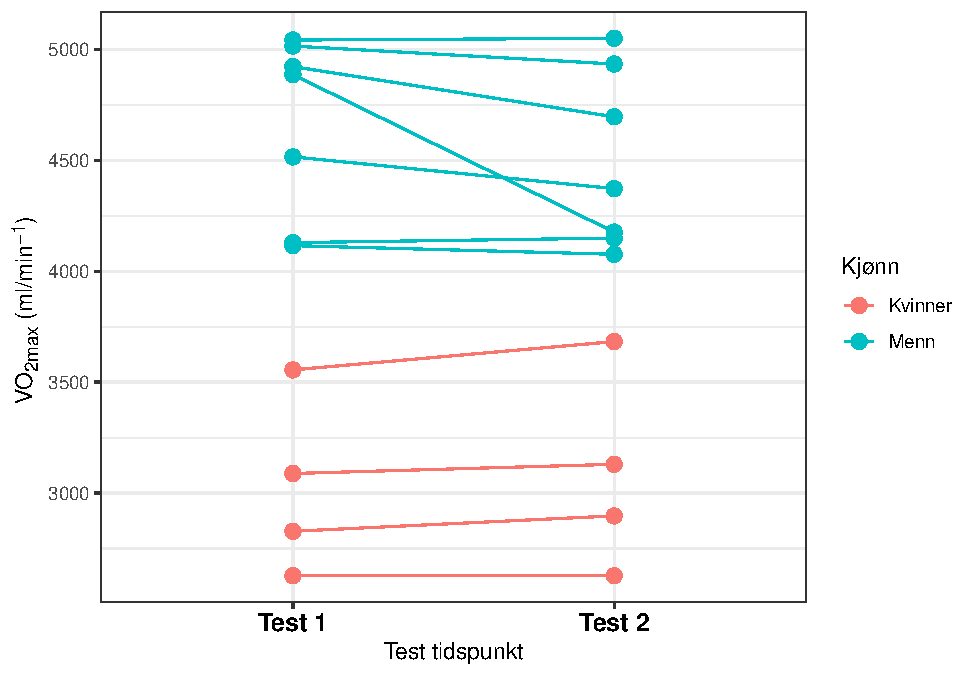
\includegraphics{_main_files/figure-latex/unnamed-chunk-3-1.pdf}
\caption{Figuren viser forskjellen i vo2max (ml/min) mellom test 1 og
test 2}
\end{figure}

\hypertarget{diskusjon}{%
\section{Diskusjon}\label{diskusjon}}

Resultatet i vårt reabilitetstudie er at typefeil er på 4.04\%.
Typefeilen kan tyde på at enkelte av disse resultatene kan være utsatt
for støy av ulik sort (\protect\hyperlink{ref-hopkins2000}{Hopkins
2000}). Ettersom testing av maksimalt oksygenopptak er en test som
gjennomføres til utmattelse, vil man kunne forvente en viss variasjon i
testresultatene ettersom opplevd anstrengelse kan påvirkes av flere
ulike variabler (\protect\hyperlink{ref-halperin2015}{Halperin, Pyne,
and Martin 2015}). For å redusere støy vil flere faktorer være nyttig å
ta hensyn til under slik testing. Som nevnt i metoden vil
standardisering av matinntak, koffeininntak, utstyr og tidspunkt for
gjennomføring av test være med på å kunne sikre intern validitet i
resultatene. Eksempler er deltakernes kjennskap til testen, verbal
oppmuntring og personer tilstede under testen er andre faktorer som
potensielt kan bidra til støy
(\protect\hyperlink{ref-halperin2015}{Halperin, Pyne, and Martin 2015}).
Felles for alle faktorer er at graden av påvirkning på resultatene
muligens reduseres ved hjelp av en standardisert testprotokoll.
Deltakerne - og testlederne, sin kjennskap til testen er en annen faktor
som trolig påvirker resultatene i vårt prosjekt. I dette tilfellet
fantes det enkelte deltakere som hadde gjennomført en liknende test
flere ganger, og en kan da forvente en mindre grad av variasjon mellom
resultatene på test 1 og test 2, sammenlignet med de deltakerne som
gjennomførte testen for første gang under test 1. Dette fordi
kjennskapen og kunnskapen de tilegnet seg på test , trolig spiller inn
på testresultatene.

Grunnen til at vi snakker om typefeil er at når vi ønsker å måle
påvirkningen av trening på en gruppe individer er det viktig å kunne si
noe om hva som er endring og hva som er støy (målefeil). Desto mindre
støy en test innebærer jo bedre er målingen. Målet som brukes er
typefeil. Hva som danner denne variasjonen som representeres ved typical
error er multifaktorelt, men hoveddelen er som oftest biologisk
(\protect\hyperlink{ref-hopkins2000}{Hopkins 2000}).

For å måle typefeil har vi brukt within subject deviation metoden. Denne
metoden påvirkes ikke av at gjennomsnittet endrer seg fra test til test
(\protect\hyperlink{ref-hopkins2000}{Hopkins 2000}). Data for målinger i
vo2max fra fem sertifiserte Australske laboratorier fastslo ett
gjennomsnitt på 2.2\% for typefeil
(\protect\hyperlink{ref-halperin2015}{Halperin, Pyne, and Martin 2015}).
Data fra det Australske institutt for sport har også fastslått at en
typefeil på omtrent 2\% er riktig for både maksimal og submaksimal
vo2max (\protect\hyperlink{ref-clark2007}{Clark et al. 2007};
\protect\hyperlink{ref-robertson2010}{Robertson et al. 2010};
\protect\hyperlink{ref-saunders2009}{Saunders et al. 2009}). Dette
indikerer at med godt kalibrert utstyr og med utøvere som er godt vant
med testingen vil en typefeil på 2\% for det biologiske, og analytiske
være riktig (\protect\hyperlink{ref-halperin2015}{Halperin, Pyne, and
Martin 2015}). Vår typefeil på 4.04\% kan derfor tenkes å være et bilde
hvordan det kan se ut med få deltakere, med ulikt utgangspunkt, men også
uten skikkelig standardisering av treningshverdagen i forkant av
testene. Det kan også tenkes at med et varierende nivå hos deltagerne
kan enkelte oppleve en treningseffekt av test 1. Samtidig som andre
kanskje ble slitne av å få en test inn i treningshverdagen.

\hypertarget{labrapport---cdna-synthesis-using-superscript-iv-and-general-qpcr}{%
\chapter{Labrapport - cDNA synthesis using Superscript IV and general
qPCR}\label{labrapport---cdna-synthesis-using-superscript-iv-and-general-qpcr}}

\hypertarget{formuxe5l}{%
\section{Formål}\label{formuxe5l}}

RNA-overflodsanalyse er gjort ved hjelp av syntese av komplementært DNA
fra enkelttrådet RNA. Vi ønsker å amplifisere opp bestemte proteiner ved
hjelp av bestemte primere og qPCR. Vi ønsker å få frem en cQ-verdi for å
kunne evaluere gen-opphopningen, og sammenlikne mål-genene med referanse
gener.

Estimere reaksjonseffektivitet Dobler mengden målgen per syklus

\hypertarget{metode-1}{%
\section{Metode}\label{metode-1}}

Vi hentet cDNA fra 3 forsøkspersoner. Dette er cDNA hentet fra testene
som ble gjennomført i uke 0 og uke 2. Alle prøver er fra venstre ben.
Det ble laget en 5 fortynningsserier fra disse prøvene. Dette ble
fortynnet ved hjelp av DEPC-behandlet vann, i følgende serie 1:10, 1:50,
1:250, 1:1250, 1:6250, 1:31250, 1:156250. Vortex ble brukt mellom hver
fortynningsfase.

Det ble derreter laget sju forskjellige master mixer ved hjelp av 3
referansegener (REEP5, CHMP2A, B2M) og 4 målgener (MyHC I, 2A, 2X, rRNA
475). Mastermix bestod av 5 µl sybr green, 1 µl valgt gen, 2 µl
DEPC-behandlet vann , 2 µl fortynnet cDNA. Deretter ble det fylt 71
brønner i en qPCR-reaksjonsplate ed henholdsvis 2 µl prøve, og 8 µl med
mastermix. Reaksjonsplaten med brønner ble dekt med plastfilm, og
sentrifugerte 1 minutt på 1200 omrdreininger (rpm), før PCR protokoll
ble gjennomført.

En PCR protokoll ble på forhånd forberedet i QuantStudio5. PCR
protokollen bestod av 50 grader i 2 minutter, og 95 grader i 2 minutter,
før den kjørte 40 sykluser bestående av 1 sekund på 95 grader celsius,
og 30 sekunder på 60 grader celsius.

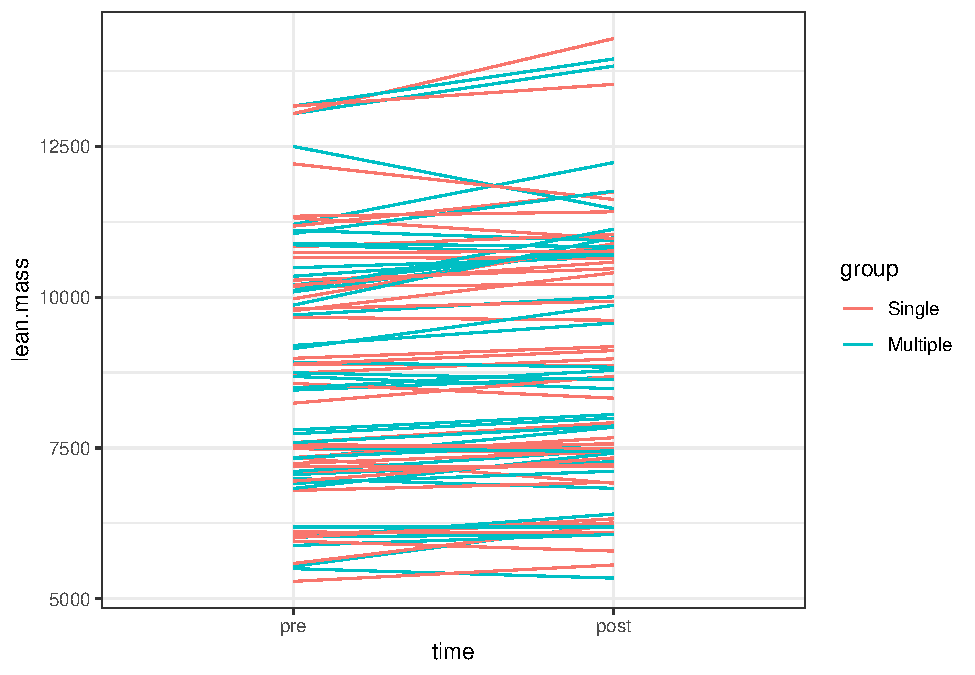
\includegraphics{_main_files/figure-latex/unnamed-chunk-5-1.pdf}

\hypertarget{resultater-1}{%
\section{Resultater}\label{resultater-1}}

Modellen viser sammenhengen mellom antall sykluser og fluorescence.
Flere PCR-sykluser gir flere kopier, og dermed også en økt konsentrasjon
i prøven. På denne måten kan vi bruke fluorescence til å si noe om hvor
mange sykluser som må til for å oppnå en bestemt terskelverdi(Cq-verdi).
Med primerne vi benyttet i forsøket var det ønskelig med et sted mellom
10 og 40 sykluser for å sikre at vi oppnådde terskelverdien. Det ble
derfor kjørt 40 sykluser.Ved flere sykluser øker trolig sannsynligheten
for falske positive.

\begin{verbatim}
## `geom_smooth()` using formula 'y ~ x'
\end{verbatim}

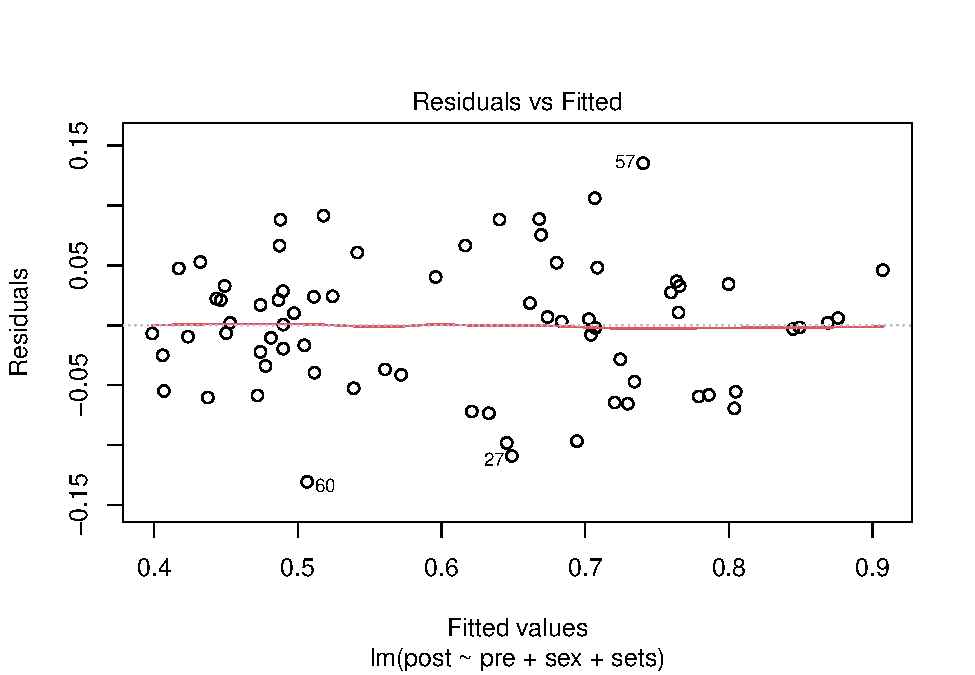
\includegraphics{_main_files/figure-latex/unnamed-chunk-6-1.pdf}

\begin{verbatim}
## `geom_smooth()` using formula 'y ~ x'
\end{verbatim}

\begin{figure}
\centering
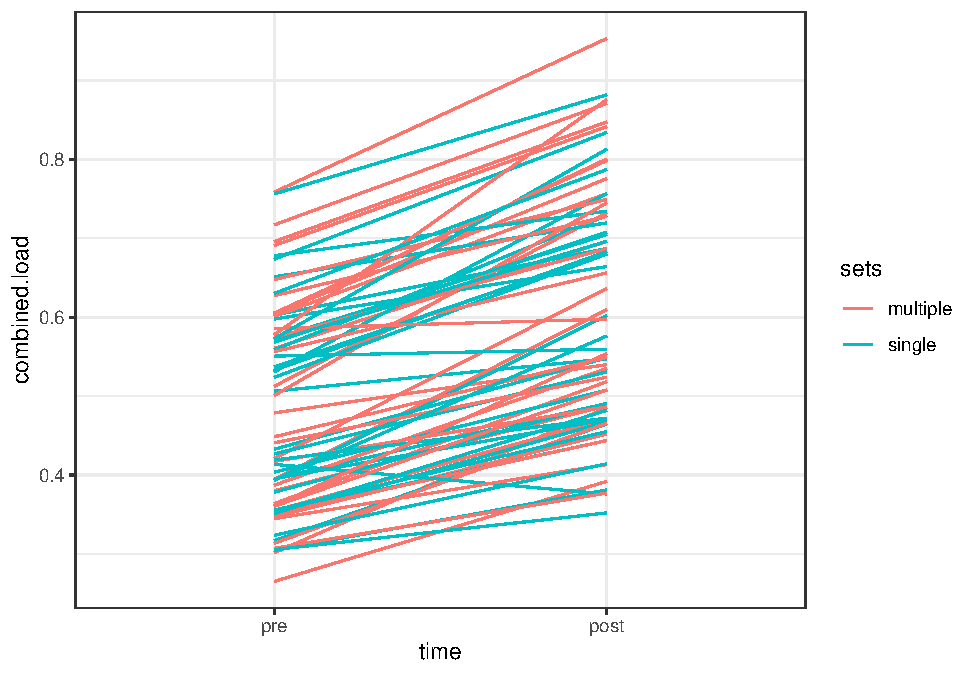
\includegraphics{_main_files/figure-latex/unnamed-chunk-7-1.pdf}
\caption{Efficiency calculations made from serial dilution of cDNA}
\end{figure}

\begin{verbatim}
## a flextable object.
## col_keys: `sample`, `time`, `MYHC1`, `MYHC2A`, `MYHC2X`, `RRNA47S`, `CHMP2A`, `REEP5`, `B2M` 
## header has 1 row(s) 
## body has 6 row(s) 
## original dataset sample: 
##   sample time MYHC1 MYHC2A MYHC2X RRNA47S CHMP2A REEP5   B2M
## 1    FP1   w0 19.53  20.03  22.87   24.88  26.68 26.68 23.79
## 2    FP2   w0 19.70  20.04  29.80   27.54  26.78 26.59 25.22
## 3    FP3   w0 20.33  18.25  22.87   25.27  25.97 26.55 24.53
## 4    FP1   w2 19.96  17.59  26.01   32.36  26.73 26.87 24.01
## 5    FP2   w2 20.20  14.64  26.23   27.00  26.45 26.40 24.56
\end{verbatim}

\hypertarget{diskusjon-1}{%
\section{Diskusjon}\label{diskusjon-1}}

Cq-verdien sier noe om hvor mange PCR-sykluser som trengs for å
detektere ulike målgen(\protect\hyperlink{ref-kuang2018}{Kuang et al.
2018}). En høyere Cq-verdi indikerer altså at mengden RNA må dobles
flere ganger for å detektere en terskelverdi av target. En lavere
Cq-verdi indikerer at terskelverdien oppnås ved færre PCR-sykluser,
altså at konsentrasjonen av target er høyere. En lavere Cq-verdi ved uke
2, sammenlignet med uke 0(baseline) som i forsøket, indikerer høyere
konsentrasjon ved uke 2 enn ved uke 0. Dermed en effekt av
intervensjonen, avhengig av funksjonen til målgenet vi underøkser.

\hypertarget{arbeidskrav-i-vitenskapsteori}{%
\chapter{Arbeidskrav i
vitenskapsteori}\label{arbeidskrav-i-vitenskapsteori}}

\hypertarget{oppgave-1}{%
\section{Oppgave 1}\label{oppgave-1}}

Falsifikasjonisme Karl Popper var en analytisk filosof, som utarbeidet
et falsifiserbarhetskriterium. Popper ble inspirert til denne
tankegangen gjennom tre ulike kilder, demarkasjonsproblemet,
induksjonsproblemet og risikable forutsigelser. Demarkasjonsproblemet
danner grunnlaget for utfordringen med å skille vitenskap og
pseudovitenskap fra hverandre. Induksjonsproblemet stiller et spørsmål
om hvordan man kan vite at en vitenskapelig teori er sann. Dette så ikke
Popper på som et problem da han mente at vitenskapelige teorier ikke kan
bekreftes. Det siste som inspirerte popper er risikable forutsigelser
som er vanskelig eller umulige å falsifisere
(\protect\hyperlink{ref-alnes2018}{Alnes 2018}).

Poppers demarkasjonskriterium kommer fra ønsket å skille vitenskapelig
teori fra ikke-vitenskapelig teori også kalt pseudovitenskap
(\protect\hyperlink{ref-dellsuxe9n2021}{Dellsén 2021}). Løsningen på
dette mente han ikke kunne komme fra å verifisere teorier, da dette kan
være vanskelig eller umulig. Løsningen på dette problemet blir da å
falsifisere teorier, ergo å bekrefte at de er usanne, eller feil. Et
eksempel på dette er en teori om at alle hunder er hvite. Det er umulig
å bekrefte at det aldri har vært hunder som har en annen farge, eller at
det noen gang kommer til å være hunder som har en annen farge. Dette er
årsaken til at Popper mener det er umulig å bekrefte en teori, da man
aldri kan vite hva som har vært eller hva som kommer. Ved å bruke samme
eksempel kan man falsifisere teorien når man oppdager en hund som ikke
er hvit. Falsifikasjon er da kriteriet som kan skille vitenskap fra
pseudovitenskap, i følge Popper
(\protect\hyperlink{ref-okasha2016}{Okasha 2016}).

Popper ytret at vitenskapelige teorier som ikke er mulig å falsifisere,
hvor man uansett kan få de empiriske bevisene til å passe inn i teorien,
skaper lite troverdighet og at disse ikke skulle godtas som
vitenskapelig teori (\protect\hyperlink{ref-okasha2016}{Okasha 2016}).
Popper (\protect\hyperlink{ref-popper1969}{Popper 1969}) forklarer dette
med teorier fra Marx, Freud og Adler, som han syns var utfordrende at
skulle aksepteres som vitenskapelige teorier. Teorier som er mulig å
falsifisere (dette betyr ikke at de trenger å være usanne) er mer
troverdig, og viktige teorier når de blir testet.

Samir Okasha (\protect\hyperlink{ref-okasha2016}{Okasha 2016}) beskriver
flere utfordringer ved Poppers falsifiserbarhetskriterium. En av
utfordringene Okasha beskriver er hvordan dette kriteriet kan påvirke
hvordan verden blir oppfattet hvis man hele tiden skal avkrefte teorier.
Med dette mener han at vitenskapelige teorier som ikke kan falsifiseres
likevel kan ha eller hatt stor påvirkning på hvordan den vitenskapelige
teoriene kan utvikle seg. Disse teoriene kan og bidra til nye viktige
oppdagelser innenfor tematikken. Videre beskriver Okasha problematikken
med å skulle definere hvile teorier som kan kalles vitenskap og
ikke-vitenskap, og hvorfor dette ikke er nødvendig. Et av eksemplene han
trekker frem er hvordan det nesten er umulig at alle observasjoner
stemmer med en vitenskapelig teori. Videre beskriver han hvor vid og
bred vitenskapen er, og hvor ulik alle teoriene er. Han beskriver
vitenskap som ulike teorier som har mange fellestrekk, og at selv uten
alle fellestrekkene vil dette være vitenskapelige teorier med
bekreftende observasjoner (\protect\hyperlink{ref-okasha2016}{Okasha
2016}). Jeg mener Okasha har et godt poeng i at det ikke er så viktig å
skille mellom vitenskap og psudovitenskap som Popper ønsket. Som Okasha
påpeker har det blitt gjort viktig oppdagelser i lyset av en teori som
viste seg å ikke stemme, og det er derfor ikke like viktig med det
markante skillet, men at begrepet er litt flytende.

\hypertarget{oppgave-2}{%
\section{Oppgave 2}\label{oppgave-2}}

HD-metoden og abduksjon/Bayesisme Hypotetisk deduktiv metode kan deles i
to ulike kontekster for ulike faser av utvikling av teorien,
oppdagelseskonteksten og begrunnelseskonteksten. Oppdagelseskonteksten
er miljøet der teorien eller hypotesen blir oppdaget. I følge Hempel
finnes det ingen bestemt metode å finne opp nye ideer, men de kan for
eksempel oppstå fra fantasier eller ulike observasjoner man gjør
(\protect\hyperlink{ref-dellsuxe9n2021}{Dellsén 2021}). Dette kan
forekommer tilfeldig, eller hvis man prøver å finne en forklaring eller
årsak på et bestemt problem. Dette er begrunnelseskonteksten. Hempel
(\protect\hyperlink{ref-hempel1966}{Hempel 1966}) beskriver at det ikke
er noen fasit på hvordan nye teorier blir oppdaget, men at det skje på
mange ulike måter.

Den logiske strukturen i hypotetisk deduktiv metode er å bekrefte om en
idé stemmer ved å teste den, gjennom å observere konsekvensene. Metoden
er delt inn i fire ulike faser for bekreftelse av en ny teori
(\protect\hyperlink{ref-dellsuxe9n2021}{Dellsén 2021}). Fase en er å
oppdage en ny teori eller lete etter en hypotese på et problem. Andre
fase er å dedusere de empiriske konsekvensene fra teorien. Dette vil si
at hypotesen kan være «det finnes liv på Jupiter». Dette vil si at de
empiriske konsekvensene av dette vil være at det er oksygen på Jupiter,
det er vann på Jupiter osv. Ved fase 3 undersøker man, og samler inn
data for å se om hypotesen stemmer, og om innsamlede data stemmer med de
empiriske konsekvensene. For eksempelet beskrevet over vil dette bety at
man må teste om det er oksygen, vann osv på Jupiter. Hvis de ikke
stemmer forkaster man, eller endre hypotesen for å komme nærmere en ny
idé eller hypotese som forklarer problemstillingen. Når man eventuelt
har innsamlede data som stemmer med de empiriske konsekvensene kan man
konkludere. Da har man til en viss grad fått en induktiv bekreftelse av
hypotesen. Dette fordi det kan være andre årsaker som fører til
endringen eller årsakssammenheng som hypotesen ikke tar for seg. Dette
vil ikke bety at den hypotesen som man først har kommet frem til ikke
stemmer, men at det er andre årsaksforhold som og kan påvirke
(\protect\hyperlink{ref-hempel1966}{Hempel 1966}).

Abduksjon er en vitenskapelig metode man bruker for å bekrefte teorier.
Denne metoden handler om å dra slutninger til den beste forklaringen til
et nytt fenomen eller ny data. For å finne dette trenger man flere ulike
teorier som har forskjellige årsaksforklaringer på dataen. Det er flere
elementer som kan bidra til at en forklaring er bedre. Hvis teorien har
forklaringskraft, forklarer flere forskjellige data, vil dette styrke
teorien. Det samme gjelder hvis teorien har en enklere årsaksforklaring,
forklarer dataen ut fra færre ting
(\protect\hyperlink{ref-dellsuxe9n2021}{Dellsén 2021}). Dette vil si at
i abduksjon må man sammenligne flere ulike forklaringer til samme
fenomen, og finne den som best forklarer dataen.

For å sammenligne med hypotetisk deduksjon som oppgir en hypotese med
ulike empiriske konsekvenser tilbyr abduksjon flere hypoteser eller
forklaringer. Noe som kan være en svakhet med HD metoden er at det kan
være flere konsekvenser og årsaker som kan underligge ved en «korrekt»
hypotese enn det man ser. En annen svakhet med HD metoden er at svarene
man får fra dataen kan være en tilfeldighet, som gjør at det virker som
man bekrefter hypotesen, men det er egentlig andre bedre forklaringer på
problemet. Dette er et av problemene som gjorde at abduksjon ble skapt.
Ved abduksjon ønsker man å se på ulike forklaringer og finne den metoden
som gir den beste forklaringen til problemet. Dette betyr at det
abduksjon ønsker å se flere forklaringene til det samme problemet for å
finne den beste forklaringen
(\protect\hyperlink{ref-dellsuxe9n2021}{Dellsén 2021}).

\hypertarget{oppgave-3}{%
\section{Oppgave 3}\label{oppgave-3}}

Bird beskriver replikasjonskrisen som foregår innenfor forskningsfeltet,
som et stort problem som kan ha flere negative konsekvenser for
vitenskapelig allmenhet, som at troverdigheten er synkende. Bird bruker
tre ulike konsept for å forklare replikasjonskrisen. Disse er type-I
feil, type-II feil og basefrekvensfeilen. Type-I feil, er å akseptere en
hypotese eller teori som ikke stemmer
(\protect\hyperlink{ref-bird2020}{Bird 2020}). Et eksempel på dette kan
være en promilletest som viser at en sjåfør kjører med promille, selv om
sjåføren ikke har drukket alkohol. Type-II feil er å forkaste en
hypotese eller en teori som faktisk stemmer. Dette kan være at en
promille test viser at en påvirket sjåfør ikke har promille.
Basefrekvensfeilen er en feil som forekommer når man fokuserer på at en
viss sannsynlighet forekommer ved en test, som å se på hvor mange
sjåfører som kjører ruspåvirket. Hvis 50 av 1000 mennesker som blir
testet for rus, tester positivt, men bare 10 faktisk kjørte ruspåvirket,
vil det si at det var 40 falsk-positive tester. Fenomenet påpeker da at
når man konkluderer med hvor mange tester som slo ut for rus, og ikke
tar hensyn for hvor mange falsk-positive tester det var forekommer
basefrekvensfeilen. Det er færre folk som ikke kjører påvirket, så da er
sannsynligheten for at de daller i den 5\% feilen større enn at de
faktisk kjører ruspåvirket. I dette eksempelet vil basefrekvensfeilen
oppstå fordi frekvensen av ruspåvirket sjåfører mot ikke-ruspåvirket
sjåfører i befolkningen generelt er lav. Bird påpeker hvordan dette slår
ut i forskning ved å bruke dette fenomenet. Satt i sammenheng med
forskning viser Bird til hvordan dette vil slå ut på hypotesetesting, og
hvordan falsk-positive, og falsk-negative forkastninger vil forekomme.
Dette fordi man ikke tar høyde for den generelle forekomsten i
befolkningen når man tester på for små grupper
(\protect\hyperlink{ref-bird2020}{Bird 2020}).

En annen forklaringer som blir nevnt ved replikasjonskrisen er
publikasjons bias. Publikasjons bias forekommer når resultater blir
skjevt fremstilt for å avgjøre om en studie skal publiseres eller ikke.
Dette forekommer først og fremst ved å oftere publisere studier med
statistisk signifikante resultater. Dette vil da bety at studier som er
gjennomført hvor resultatene ikke er statistisk signifikante,
resultatene ikke stemmer med hypotesen ikke vil bli publisert
(\protect\hyperlink{ref-bird2020}{Bird 2020}).

Andre forklaringer til replikasjonskrisen er at flere studier ikke blir
gjennomført på tilstrekkelig måte for å kunne repetere forsøket, eller
at studiet mangler validitet, ergo at studiet ikke gjennomføres på den
måten det var planlagt at det skulle gjøres, eller gjennomført slik det
er beskrevet at det er gjort. En annen forklaring som blir nevnt er
hacking av resultater for å få en studie til å se bedre ut enn det er
(\protect\hyperlink{ref-bird2020}{Bird 2020}).

Bird presenterer en mer akademisk forklaring enn de andre årsakene som
blir nevnt. Om forskere driver med svindel eller praktiserer dårlig
gjennomføring i studiene blir vanskelig å kunne konkludere med. Bird
kommer med en forklaring som viser hvordan hypotesetesting kan tolkes
feil, eller aksepteres med stor mulighet for type-I eller type-II feil.
Forklaringene som har blitt nevnt er alle aksepterbare, og mulige, og
det blir vanskelig å konkludere at den ene er bedre enn den andre, men
Bird presenterer en mer troverdig forklaring
(\protect\hyperlink{ref-bird2020}{Bird 2020}).

\hypertarget{styrke-og-utholdenhetstrening-for-godt-trente-syklister}{%
\chapter{Styrke og utholdenhetstrening for godt trente
syklister}\label{styrke-og-utholdenhetstrening-for-godt-trente-syklister}}

Styrketrening og utholdenhetstrening for godt trente syklister
Introduksjon I denne oppgaven skal jeg se på fem ulike
forskningsartikler som undersøke hvilken effekt styrketrening, i tillegg
til utholdenhetstrening, har på godt trente syklister. Disse fem
artiklene har jeg valgt på bakgrunn av at alle ser på hvilken effekt
styrketrening har på prestasjon i sykkel, og hvordan de har brukt ulike
metoder og tester for å vise resultatet.

\hypertarget{metode-2}{%
\section{Metode}\label{metode-2}}

\underline{\textbf{Hypotese}}

Litteraturen som er valgt til denne oppgaven har alle som hovedmål å
undersøke hvordan tung styrketrening i tillegg til vanlig
utholdenhetstrening vil påvirke ulike prestasjonsfaktorer innenfor
sykling. Hvilke prestasjonsfaktorer som blir vektlagt varierer mellom de
ulike forskningsartiklene. Rønnestad
(\protect\hyperlink{ref-ruxf8nnestad2010b}{Bent R. Rønnestad, Hansen,
and Raastad 2010a}) presenterer sin hypotese at styrketreningen vil
påvirke muskeltverrsnitt i lårmuskulaturen, power output, windgate test,
og 40 min all-out test. Vikmoen et al
(\protect\hyperlink{ref-vikmoen2016}{Vikmoen et al. 2016}) presenterer
samme hypotese, men studien gjennomføres kun på kvinnelige
elitesyklister. I artikkelen fra
(\protect\hyperlink{ref-ruxf8nnestad2010a}{Bent R. Rønnestad, Hansen,
and Raastad 2010b}) har Rønnestad et al en hypotese om at vedlikehold av
tung styrketrening gjennom starten av treningssesongen vil positivt
påvirke utholdenheten over lengre konkurranser i slutten av en 13 ukers
periode. Dette minner om hypotesen Aagaard 2011 legger frem, men
intervensjonen og resultater blir gjennomført i forberedelses sesong, og
ikke i konkurransesesong. Siste artikkel har en hypotese som sier at 10
uker med tung styrketrening sammen med utholdenhetstrening, og 15 uker
med vedlikehold av styrketreningen vil gi økt styrke i pedaltråkk og øke
styrken i benmuskulaturen (\protect\hyperlink{ref-ruxf8nnestad2015}{B.
R. Rønnestad et al. 2015}).

\begin{longtable}[]{@{}
  >{\raggedright\arraybackslash}p{(\columnwidth - 10\tabcolsep) * \real{0.14}}
  >{\raggedright\arraybackslash}p{(\columnwidth - 10\tabcolsep) * \real{0.13}}
  >{\raggedright\arraybackslash}p{(\columnwidth - 10\tabcolsep) * \real{0.10}}
  >{\raggedright\arraybackslash}p{(\columnwidth - 10\tabcolsep) * \real{0.12}}
  >{\raggedright\arraybackslash}p{(\columnwidth - 10\tabcolsep) * \real{0.20}}
  >{\raggedright\arraybackslash}p{(\columnwidth - 10\tabcolsep) * \real{0.32}}@{}}
\toprule
\begin{minipage}[b]{\linewidth}\raggedright
\end{minipage} & \begin{minipage}[b]{\linewidth}\raggedright
Studie design
\end{minipage} & \begin{minipage}[b]{\linewidth}\raggedright
Deltakere
\end{minipage} & \begin{minipage}[b]{\linewidth}\raggedright
Intervensjon
\end{minipage} & \begin{minipage}[b]{\linewidth}\raggedright
Fysiske tester
\end{minipage} & \begin{minipage}[b]{\linewidth}\raggedright
Statistiske tester
\end{minipage} \\
\midrule
\endhead
\protect\hyperlink{ref-ruxf8nnestad2010a}{Bent R. Rønnestad, Hansen, and
Raastad} (\protect\hyperlink{ref-ruxf8nnestad2010a}{2010b}) & RCT & n=23
& 12 Uker & Benpress

Laktatprofil

Vo2 maks

Windgate

40 min all-out & Uparret t-test

To-veis ANOVA med Bonferroni post hoc \\
\protect\hyperlink{ref-ruxf8nnestad2010b}{Bent R. Rønnestad, Hansen, and
Raastad} (\protect\hyperlink{ref-ruxf8nnestad2010b}{2010a}) & RCT & n=12
& 25 Uker & Benpress

Laktatprofil

Vo2 maks

Windgate

40 min all-out & Uparret t-test \\
\protect\hyperlink{ref-ruxf8nnestad2015}{B. R. Rønnestad et al.}
(\protect\hyperlink{ref-ruxf8nnestad2015}{2015}) & RCT & n=16 & 25 Uker
& Benpress

Laktatprofil

Vo2 maks

Windgate

40 min all-out & Uparret t-test

To-veis ANOVA med post-hoc \\
\protect\hyperlink{ref-aagaard2011}{Aagaard et al.}
(\protect\hyperlink{ref-aagaard2011}{2011}) & RCT & n=14 & 16 Uker & 5
min prestasjonstest

45 min kapasitets test & Ikke-parametisk ANOVA \\
\protect\hyperlink{ref-vikmoen2016}{Vikmoen et al.}
(\protect\hyperlink{ref-vikmoen2016}{2016}) & RCT & n=21 & 11 Uker & Vo2
maks test

40 min all-out

Windgate & Uparret t-test \\
\bottomrule
\end{longtable}

\emph{Tabell 1:} Viser informasjon om studiedesing, deltakere,
treningsintervensjon og tester

\underline{\textbf{Studie design}}

Forskningsartiklene som er brukt i denne oppgaven har som hovedmål å
finne ut hvordan styrketrening, sammen med utholdenhetstrening, påvirker
profesjonelle eller godt trente syklisters prestasjon. Felles for alle
studiene er at de gjennomføre en styrkeintervensjon fra 11 til 25 uker
på intervensjonsgruppene, og sammenligner forskjellene i ulike styrke-
og utholdenhetstester med en kontrollgruppe. De sammenligner Dette vil
si at alle studiene bruker randomisert kontrollert studie (RCT) som
studiedesign. I et RCT blir deltakerne tilfeldig valgt hvilken gruppe de
tilhører, kontrollgruppe eller intervensjonsgruppe. Ved å tilfeldig
fordele de ulike deltakerne i kontrollgruppe, og intervensjonsgruppe vil
man minske sannsynligheten for at det er store forskjeller mellom
gruppene (\protect\hyperlink{ref-hulley2013}{Hulley et al. 2013};
\protect\hyperlink{ref-Parab2010}{Parab and Bhalerao 2010}). Det er med
fordel at alle studiene i denne oppgaven bruker dette studie designet
for å kunne se effekten for intervensjonsgruppen, mot kontrollgruppen.
Dette vil si at resultatene vil vise hvilken effekt intervensjonen har
eller ikke har, og ikke være påvirket av store gruppeforskjeller
(\protect\hyperlink{ref-helsebiblioteket}{Helsebiblioteket, n.d.}).

\underline{\textbf{Utvalg}}

I de ulike studiene skilte deltaker gruppene seg fra 12 til 23
deltakere. Alle deltakerne var godt trente syklister. I noen av
prosjektene var deltakerne syklister på høyt nasjonalt eller
internasjonalt nivå (\protect\hyperlink{ref-ruxf8nnestad2010a}{Bent R.
Rønnestad, Hansen, and Raastad 2010b},
\protect\hyperlink{ref-ruxf8nnestad2010b}{2010a};
\protect\hyperlink{ref-ruxf8nnestad2015}{B. R. Rønnestad et al. 2015};
\protect\hyperlink{ref-aagaard2011}{Aagaard et al. 2011}). Ingen av
forfatterne beskrev rekrutteringsprosessen eller at det ble gjennomført
en styrkeberegning (antall beregning) for å argumentere for antall
deltakere i studiene.

\underline{\textbf{Tester}}

Alle forskningsprosjektene gjennomført av Rønnestad
(\protect\hyperlink{ref-ruxf8nnestad2010a}{Bent R. Rønnestad, Hansen,
and Raastad 2010b}, \protect\hyperlink{ref-ruxf8nnestad2010b}{2010a};
\protect\hyperlink{ref-ruxf8nnestad2015}{B. R. Rønnestad et al. 2015})
gjennomfører de samme fysiske testene for å teste intervensjonsgruppen
mot kontrollgruppen. Disse testene er beskrevet i tabell 1. Vo2 maks
test, windgate og 40 min all-out test ble brukt i prosjektet gjennomført
av Vikmoen (\protect\hyperlink{ref-vikmoen2016}{Vikmoen et al. 2016}). I
det siste prosjektet ble det gjennomført en 5 min prestasjonstest for å
se på effekten av intervensjonen ved kort utholdenhetsprestasjon
(\protect\hyperlink{ref-aagaard2011}{Aagaard et al. 2011}). Det ble og
gjennomført en 45 min utholdenhetstest. Felles for alle
forskningsprosjektene er at testene var standardisert, for å øke
validiteten. Deltakerne måtte følge visse regler under testdagene slik
at de eksterne faktorene skulle være så like som mulige. Dette innebar
regulasjoner på inntak av mat og drikke, og trening under testdagene.
Testtidspunkt var standardisert til den enkelte deltaker, slik at
testene ble gjennomført likt på dagen, og temperaturen i testrommet var
standardisert på alle utøverne.

De ulike artiklene har brukt forskjellige statistiske tester, for å
regne ut forskjellen mellom gruppene. For å regne ut forskjellen mellom
gruppene ved pre-test har fire av prosjektene brukt uparret t-test
(\protect\hyperlink{ref-ruxf8nnestad2010a}{Bent R. Rønnestad, Hansen,
and Raastad 2010b}, \protect\hyperlink{ref-ruxf8nnestad2010b}{2010a};
\protect\hyperlink{ref-ruxf8nnestad2015}{B. R. Rønnestad et al. 2015};
\protect\hyperlink{ref-vikmoen2016}{Vikmoen et al. 2016}). En t-test
blir brukt for å regne ut om det er signifikant forskjell mellom
gjennomsnittet til to grupper. I disse studiene er t-testen brukt på to
uavhengige grupper, som gjør at man må bruke en uparet t-test
(\protect\hyperlink{ref-kim2015}{Kim 2015}). I motsetning til de andre
har Aagaard (\protect\hyperlink{ref-aagaard2011}{Aagaard et al. 2011})
gjennomført en ikke parametisk ANOVA analyse for å regne ut forskjellen
mellom gruppene ved pre-test. Ikke parametiske analyser brukes for å
sammenligne data som ikke møter standarden for nomralditrubisjon, eller
for mindre grupper som Aagaard har (n=14)
(\protect\hyperlink{ref-altman2009}{Altman and Bland 2009}). Enveis
ANOVA er en variasjonsanalyse som regner ut forskjellen i gjennomsnitt
mellom to ulike grupper grupper. Hvis dette gir en p-verdi som er lavere
enn det gitte signifikans nivået kan man konkludere med at det er
forskjell mellom gruppene, men man kan ikke si hvilken forskjell det er.
For å finne denne må man gjennomføre en post hoc test for å finne hvilke
grupper som er ulike
(\protect\hyperlink{ref-kim2017}{\textbf{kim2017?}}) . For å regne ut
den relative forskjellen mellom intervensjonsgruppen og kontrollgruppen
har Aagard også brukt en ikke-parametisk ANOVA med post hoc. Vikmoen
(\protect\hyperlink{ref-vikmoen2016}{Vikmoen et al. 2016}) og Rønnestad
(\protect\hyperlink{ref-ruxf8nnestad2015}{B. R. Rønnestad et al. 2015})
brukte uparet t-test for å regne ut relativ forskjell mellom gruppene.
Rønnestad (\protect\hyperlink{ref-ruxf8nnestad2010a}{Bent R. Rønnestad,
Hansen, and Raastad 2010b},
\protect\hyperlink{ref-ruxf8nnestad2010b}{2010a}) gjennomførte en toveis
ANOVA med Bonferroni for å regne ut den relative forskjellen ved
post-test. Ved å bruke bonferroni vil de slippe å gjennomføre flere
t-tester og få flere p-verdier som vil være vanskelig å holde styr på.

\hypertarget{resultat}{%
\section{Resultat}\label{resultat}}

Rønnestad presenter resultater med gjennomsnittig kraftutvikling i 40
min all-out testen økte i forbredelsesperioden for både
intervensjonsgruppen (8 ± 2\%, p\textless0,05) og kontrollgruppen (4 ±
1\%, p\textless0.05). Det var ingen signifikant forkjell i endring
mellom gruppene. Fra pre-test til post-test hadde intervensjonsgruppen
større endring i 40 min all-out (14 ± 3\%, p\textless0,05) enn
kontrollgruppen (4 ± 1\%, p\textless{} 0,05). Dette stemmer med
hypotesen de la frem i studiet
(\protect\hyperlink{ref-ruxf8nnestad2010a}{Bent R. Rønnestad, Hansen,
and Raastad 2010b}).

I den andre undersøkelsen av Rønnestad fra 2010 viser resultatene at
muskeltversnittet til intervensjonsgruppen økte signifiknat fra pre til
post test etter endt intervensjon (4.6 ± 0.5\%, p \textless{} 0.01), og
kontrollgruppen hadde ingen endring. Ved 40 min all-out testen var det
ingen signifikant endring mellom gruppene. Dette vil si at deler av
hypotesen stemmer med resultatene som ble funnet
(\protect\hyperlink{ref-ruxf8nnestad2010b}{Bent R. Rønnestad, Hansen,
and Raastad 2010a}).

I prosjektet hvor Rønnestad undersøkte hvordan styrke påvirker
pedaltråkk viser resultatene at endringene i maksimal styrke var større
gjennom hele testperioden for intervensjonsgruppen fra 65.8 ± 8.1 kg til
66.9 ± 8.0 kg, P \textless{} 0.05) enn for kontrollgruppen, (74.6 ± 7.1
kg til 75.9 ± 7.2 kg, P \textless{} 0.05). Det var og en signifikant
endring mellom gruppene på 40 min all-out testen (6.5 ± 5.7\%, P
\textless{} 0.01). Disse resultatene er med på å underbygge at hypotesen
stemmer (\protect\hyperlink{ref-ruxf8nnestad2015}{B. R. Rønnestad et al.
2015}).

Aagaard finner i sitt studie økte intervensjonsgruppen prestasjonen med
8\% på 45 min prestasjonstesten (313.7± 45.9 til 340.1± 33.1 W,
p\textless0,05). Forskjellen i endring i prestasjonstesten mellom
kontrollgruppen og intervensjonsgruppen var statistisk signifikant
(p\textless0,001) (\protect\hyperlink{ref-aagaard2011}{Aagaard et al.
2011}). Dette stemmer med hypotesen som ble lagt frem før studien ble
gjennomført. Intervensjonsgruppen hadde en økning 6,4\% ± 7,9 \% på 40
minutters prestasjonstest.

I studiet gjennomført på kvinner viser resultatene viser ingen
signifikant forskjell mellom gruppene. Dette viser at hypotesen
forfatterne presenterte i starten av studien ikke stemmer med
resultatene etter endt intervensjon. Dette vil si at det ikke er en
signifikant forskjell mellom kontrollgruppen som kun gjennomførte
utholdenhetstrening, og intervensjonsgruppen som gjennomførte styrke og
utholdenhetstrening (\protect\hyperlink{ref-vikmoen2016}{Vikmoen et al.
2016}).

\hypertarget{konklusjon}{%
\section{Konklusjon}\label{konklusjon}}

Flere at forfatterne kan konkludere med at hypotesen og resultat stemmer
(\protect\hyperlink{ref-aagaard2011}{Aagaard et al. 2011};
\protect\hyperlink{ref-ruxf8nnestad2015}{B. R. Rønnestad et al. 2015};
\protect\hyperlink{ref-ruxf8nnestad2010a}{Bent R. Rønnestad, Hansen, and
Raastad 2010b}). I disse studiene viser forfatter at hypotesen de har
lagt frem før gjennomført studie stememr med hovedfunnene i studiene.
Dette vil si at tung styrketrening i tillegg til utholdenhetstrening har
en positiv effekt på prestasjonsfaktorer i sykkel. Rønnestad
(\protect\hyperlink{ref-ruxf8nnestad2010b}{Bent R. Rønnestad, Hansen,
and Raastad 2010a}) sine hovedfunn viser at deler av hypotesen stemmer
med resultatene. Hypotesen om at lårmuskulaturens tverrsnitt vil øke,
stemmer med resultatene, men de kan ikke konkludere med at
intervensjonen har en effekt på 40 min all-out test. På den andre siden
viser resultatene til vikmoen
(\protect\hyperlink{ref-vikmoen2016}{Vikmoen et al. 2016}) at hypotesen
og resultat ikke stemmer, og kan ikke konkludere med at
treningsintervensjonen har den forventede effekten.

\hypertarget{styrketrening-med-ett-sett-vs-tre-sett}{%
\chapter{Styrketrening med ett sett vs tre
sett}\label{styrketrening-med-ett-sett-vs-tre-sett}}

\hypertarget{introduksjon-1}{%
\section{Introduksjon}\label{introduksjon-1}}

Flere forskere har undersøkt forskjellen på hvordan ulike sett og reps
påvirker maksimal styrke, muskel hypertrofi og kroppssammensetning.
Schoenfeld og flere {[}schoenfld2019{]} gjennomførte et studie for
undersøke forskjellen i hypertrofi forskjellen mellom å gjennomføre ett
eller tre sett i styreprogrammet. I denne studien var det ingen
signifikant forskjell mellom gruppen som gjennomførte ett sett og
gruppen som gjennomførte tre sett, men begge gruppene hadde signifikant
økt muskel styrke fra pre-test til post-test. Flere andre gjennomførte
studier viser et annet resultat, og konkluderer med at å gjennomføre tre
sett gir en statistisk signifikant økning i maksimal styrke
(\protect\hyperlink{ref-rhea2002}{Rhea et al. 2002};
\protect\hyperlink{ref-munn2005}{Munn et al. 2005};
\protect\hyperlink{ref-fruxf6hlich2010}{Fröhlich, Emrich, and
Schmidtbleicher 2010}). På den andre siden konkluderer Carpinelli
(\protect\hyperlink{ref-carpinelli1998}{Carpinelli and Otto 1998}), at
det ikke er signifikant forskjell på ett og tre sett, og diskuterer for
at ett sett holder for å få god utvikling i muskelstyrke.

Dette danner grunnlaget for ønsket om å undersøke denne
problemstillingen videre. Formålet med denne studien er å se om det vil
forekomme endring i lean bodymass og styrkeadaptasjon etter 12 ukers
treningsintervensjon, med ulik volum belastning på hvert ben, og
sammenligne disse endringene.

\underline{\textbf{Intervensjon}}

Intervensjonen bestod av 12 ukers full-kropps styrketrening.
Beinøvelsene ble gjennomført på et og et bein for å tillate interne
styrkeforskjeller. Begge utøverne gjennomførte begge protokollene (et
sett, og tre sett) og det ble tilfeldig valgt hvilket ben som skulle
gjennomføre hvilken protokoll. Muskelstyrken ble vurdert ved oppstart,
under (uke 3,5 og 9) og etter treningsintervensjon. Kroppssammensetning
ble målt før og etter treningsintervensjonen. Muskelbiopsi ble samlet 4
ganger under intervensjonen. Ved start av intervensjon, før, og en time
etter treningsøkt fem, og etter intervensjon.

\underline{\textbf{Treningsprotokoll}}

\underline{\textbf{Oppvarming}}

Alle deltakerne gjennomførte en standardisert oppvarmingsprotokoll før
hver treningsøkt, hvor protokollen bestod av tre deler. Første del
bestod av 5 min sykling på ergometersykkel til opplevd anstrengelse på
12-14 på Borg-skalaen (RPE). Andre del av oppvarmingen 10 repetisjoner
av fire kroppsvekt treningsøvelser (individuelt tilpasset armhevninger,
sit-ups, rygghev og knebøy). Siste del av oppvarmingen var et sett med
10 repetisjoner av \textasciitilde50\% av en repetisjon maksimum (RM),
for hver motstandsøvelse.

\underline{\textbf{Styrkeprogram}}

Beinøvelsene ble gjennomført i denne rekkefølgen: et beins beinpress,
knefleksjon og kneekstensjon. Disse ble gjennomført som et eller tre
sett per øvelse. Det ene settet ble gjennomført mellom andre og tredje
sett. Etter å ha beinøvelsene gjennomførte deltakerne benkpress med
manualer, nedtrekk og skulderpress eller sittende roing. Pausene mellom
settene var 90-180 sekunder. Treningsintensiteten økte gradvis gjennom
de 12 ukene. Deltakerne startet med 10RM de første to ukene, 8RM de
neste tre ukene, og 7RM de siste sju ukene.

\underline{\textbf{Tester}}

\underline{\textbf{Maksimal styrke}}

Maksimal styrke ble vurdert som 1RM i benpress med manualer og
kneekstensjon. Spesifikk oppvarming på testdagen bestod av 10, 6 og 3
repetisjoner på 50, 75 og 85 \% av forventet maksimum. 1RM ble funnet
ved å øke motstanden gradvis inntil deltakeren ikke klarte å gjennomføre
en fullstendig repetisjon. På hver øvelse ble den høyeste vekten
deltakeren klarte å fullføre godkjent som 1RM. Deltakerne fikk fire til
seks forsøk hver.

\underline{\textbf{Kroppssammensetning}}

Kroppssammensetningen ble testet før og etter intervensjonen ved bruk av
dual-energy røntgenabsorptiometri (DXA), i henhold til standard
protokoll. Før DXA-målingene fikk deltakerne beskjed om å faste i 2
timer, og ikke gjennomføre moderat fysisk aktivitet 48 timer før
testtidspunkt. Den siste DXA-målingen ble gjennomført to dager etter
siste styrkeøkt.

\underline{\textbf{Statistisk test}}

Statistisk analyse er gjennomført i R-studio (Version 1.4.1717).
Deskriptiv statistikk er oppgitt som prosent, og ANCOVA modell er brukt
til å regne ut p-verdi på endringsscore fra pre- til post-test.
Statistisk signifikans er satt ved p \textless0,05.

\hypertarget{resultater-2}{%
\section{Resultater}\label{resultater-2}}

\underline{\textbf{Lean bodymass}}

Resultatene presentert i studien viser at 12 uker med styrketrening
førte til en endring av lean body mass fra pre til post test på beina
som gjennomførte tre sett (3,32 ± 4,39\%, p\textless0,001), det samme
gjelder for beina som gjennomførte ett sett (2,04 ± 3,71\%,
p\textless0,001). Endringer mellom de ulike treningsintervensjonene
viser ingen signifikant endring mellom gruppene (114,56 ae,
p\textless0,193).

\underline{\textbf{Muskel styrke}}

Resultatene viser at 12 ukers treningsintervensjon fører til en endring
i muskelstyrke fra pre til post test på beina som gjennomførte et sett.
mellom beina som gjennomførte ett sett (31,0 ± 14,2\%, p\textless0,001),
og beina som gjennomførte tre sett (2,04 ± 3,71\%, p\textless{} 0,001).
Endring i muskelstyrke for de ulike treningsintervensjonene ved post
test er signifikant (p\textless0.029).

\begin{figure}
\includegraphics[width=1.2\linewidth]{_main_files/figure-latex/unnamed-chunk-11-1} \caption{Figuren viser økning i muskelstyrke mellom ett-sett og tre-sett ved pre- og post-test etter 12 uker med styrketrening (diff= -0.029AU)}\label{fig:unnamed-chunk-11}
\end{figure}

\hypertarget{diskusjon-2}{%
\section{Diskusjon}\label{diskusjon-2}}

To til tre styrkeøkter i 12 uker øker maksimal styrke i beina, og muskel
hypertrofi. Disse resultatene er gjeldende for om man gjennomfører ett
eller tre sett. Resultatene presentert i denne studien viser at
endringen vil være større om man gjennomfører tre sett. Dette samsvarer
med det store mengder av litteraturen viser
(\protect\hyperlink{ref-rhea2002}{Rhea et al. 2002};
\protect\hyperlink{ref-munn2005}{Munn et al. 2005};
\protect\hyperlink{ref-fruxf6hlich2010}{Fröhlich, Emrich, and
Schmidtbleicher 2010}). Som presentert i introduksjonen viser
resultatene de presenterer at tre sett har signifikant større økning enn
ett sett. (Rhea \protect\hyperlink{ref-rhea2002}{Rhea et al. 2002})
viser til at deltakerne som kjørte tre sett hadde dobbelt så stor
utvikling som deltakerne som gjennomførte ett sett (25\%) etter tre uker
(48\%). Etter 12 uker ble det større forskjell mellom gruppene hvor
deltakerne som gjennomførte tre sett hadde 56\% økning, og deltakerne
som gjennomførte ett sett hadde 26\% økning. Dette kan være et tegn på
at skilnaden mellom gruppen kan være enda større hvis samme
styrkeprogram blir gjennomført i en periode som er lengre enn 12 uker.

På den andre siden konkluderer Carpinelli
(\protect\hyperlink{ref-carpinelli1998}{Carpinelli and Otto 1998}) som
nevnt i introduksjonen at forskjellen mellom deltakerne som gjennomført
ett sett og tre sett ikke var stor nok til at det var hensiktsmessig å
gjennomføre tre sett. Dette understreker de med å påpeke at ved så lite
forskjell vil det være lettere for folk å praktisere ett sett i sitt
treningsprogram i det daglige liv. Dette er et viktig poeng å ta med seg
inn i resultatene fra dette studiet da det er gjennomført på vanlige
mennesker, og ikke treningsutøvere, som kan ha vanskeligheter med å få
tid til å gjennomføre et styrkeprogram med tre sett på hver øvelse.
Resultatene presentert over viser og at beina som gjennomførte ett sett
hadde signifikant endring i lean bodymass, og i muskelstyrke.

\hypertarget{konklusjon-1}{%
\section{Konklusjon}\label{konklusjon-1}}

Etter endt studie kan man konkludere med at om man gjennomfører ett sett
eller tre sett med styrketrening to til tre ganger i uken, vil man kunne
se en signifikant økning i muskel styrke og hypertrofi. Ved å
gjennomføre tre sett vil endringen være større enn ved ett sett. Til
videre forskning kan man undersøke hvordan denne endringen vil være i en
lengre periode enn 12 uker.

\hypertarget{refs}{}
\begin{CSLReferences}{1}{0}
\leavevmode\vadjust pre{\hypertarget{ref-aagaard2011}{}}%
Aagaard, P., J. L. Andersen, M. Bennekou, B. Larsson, J. L. Olesen, R.
Crameri, S. P. Magnusson, and M. Kjaer. 2011. {``Effects of Resistance
Training on Endurance Capacity and Muscle Fiber Composition in Young
Top-Level Cyclists: Concurrent Resistance and Endurance Training.''}
\emph{Scandinavian Journal of Medicine and Science in Sports} 21 (6):
e298--307. \url{https://doi.org/10.1111/j.1600-0838.2010.01283.x}.

\leavevmode\vadjust pre{\hypertarget{ref-alnes2018}{}}%
Alnes, Jan Harald. 2018. {``falsifikasjon {\textendash}
vitenskapsteori.''} \url{http://snl.no/falsifikasjon_-_vitenskapsteori}.

\leavevmode\vadjust pre{\hypertarget{ref-altman2009}{}}%
Altman, D. G, and J M. Bland. 2009. {``Parametric v Non-Parametric
Methods for Data Analysis.''} \emph{BMJ} 338 (apr02 1): a3167--67.
\url{https://doi.org/10.1136/bmj.a3167}.

\leavevmode\vadjust pre{\hypertarget{ref-bassett2000}{}}%
Bassett, D. R., and E. T. Howley. 2000. {``Limiting factors for maximum
oxygen uptake and determinants of endurance performance.''}
\emph{Medicine and Science in Sports and Exercise} 32 (1): 70--84.
\url{https://doi.org/10.1097/00005768-200001000-00012}.

\leavevmode\vadjust pre{\hypertarget{ref-bird2020}{}}%
Bird, Alexander. 2020. {``Understanding the Replication Crisis as a Base
Rate Fallacy.''} \emph{The British Journal for the Philosophy of
Science}, December, 000--000. \url{https://doi.org/10.1093/bjps/axy051}.

\leavevmode\vadjust pre{\hypertarget{ref-borg1982}{}}%
Borg, G. A. 1982. {``Psychophysical bases of perceived exertion.''}
\emph{Medicine and Science in Sports and Exercise} 14 (5): 377--81.

\leavevmode\vadjust pre{\hypertarget{ref-carpinelli1998}{}}%
Carpinelli, Ralph N., and Robert M. Otto. 1998. {``Strength Training:
Single Versus Multiple Sets.''} \emph{Sports Medicine} 26 (2): 73--84.
\url{https://doi.org/10.2165/00007256-199826020-00002}.

\leavevmode\vadjust pre{\hypertarget{ref-clark2007}{}}%
Clark, Sally A., P. C. Bourdon, W. Schmidt, B. Singh, G. Cable, K. J.
Onus, S. M. Woolford, T. Stanef, C. J. Gore, and R. J. Aughey. 2007.
{``The effect of acute simulated moderate altitude on power, performance
and pacing strategies in well-trained cyclists.''} \emph{European
Journal of Applied Physiology} 102 (1): 45--55.
\url{https://doi.org/10.1007/s00421-007-0554-0}.

\leavevmode\vadjust pre{\hypertarget{ref-dellsuxe9n2021}{}}%
Dellsén, Finnur. 2021. {``5. Abduksjon Og Sannsynlighet: Idr4000:
Kvantitativ Metode Og Statistikk.''}
\url{https://inn.instructure.com/courses/10324/files?preview=1136189}.

\leavevmode\vadjust pre{\hypertarget{ref-fruxf6hlich2010}{}}%
Fröhlich, Michael, Eike Emrich, and Dietmar Schmidtbleicher. 2010.
{``Outcome Effects of Single-Set Versus Multiple-Set
Training{\textemdash}An Advanced Replication Study.''} \emph{Research in
Sports Medicine} 18 (3): 157--75.
\url{https://doi.org/10.1080/15438620903321045}.

\leavevmode\vadjust pre{\hypertarget{ref-halperin2015}{}}%
Halperin, Israel, David B. Pyne, and David T. Martin. 2015. {``Threats
to internal validity in exercise science: a review of overlooked
confounding variables.''} \emph{International Journal of Sports
Physiology and Performance} 10 (7): 823--29.
\url{https://doi.org/10.1123/ijspp.2014-0566}.

\leavevmode\vadjust pre{\hypertarget{ref-helsebiblioteket}{}}%
Helsebiblioteket. n.d. {``Randomisert kontrollert undersøkelse - RCT.''}
\url{https://www.helsebiblioteket.no/kunnskapsbasert-praksis/kritisk-vurdering/rct}.

\leavevmode\vadjust pre{\hypertarget{ref-hempel1966}{}}%
Hempel, C. G. 1966. {``Scientific Inquiry: Invention and Test. I c. G.
Hempel, Philosophy of Natural Science.''} In. Princeton: Prentice Hall.

\leavevmode\vadjust pre{\hypertarget{ref-hill1923}{}}%
Hill, A. V., and H. Lupton. 1923. {``Muscular Exercise, Lactic Acid, and
the Supply and Utilization of Oxygen.''} \emph{QJM} os-16 (62): 135--71.
\url{https://doi.org/10.1093/qjmed/os-16.62.135}.

\leavevmode\vadjust pre{\hypertarget{ref-hopkins2000}{}}%
Hopkins, W. G. 2000. {``Measures of reliability in sports medicine and
science.''} \emph{Sports Medicine (Auckland, N.Z.)} 30 (1): 1--15.
\url{https://doi.org/10.2165/00007256-200030010-00001}.

\leavevmode\vadjust pre{\hypertarget{ref-hulley2013}{}}%
Hulley, Stephen B., Steven R. Cummings, Warren S. Browner, Deborah G.
Grady, and Thomas B. Newman. 2013. \emph{Designing Clinical Research}.
Fourth edition. Wolters Kluwer Health/Lippincott Williams; Wilkins.
\url{http://gen.lib.rus.ec/book/index.php?md5=867478e46f78a2300a2378565916f924}.

\leavevmode\vadjust pre{\hypertarget{ref-kim2015}{}}%
Kim, Tae Kyun. 2015. {``T Test as a Parametric Statistic.''}
\emph{Korean Journal of Anesthesiology} 68 (6): 540--46.
\url{https://doi.org/10.4097/kjae.2015.68.6.540}.

\leavevmode\vadjust pre{\hypertarget{ref-kuang2018}{}}%
Kuang, Jujiao, Xu Yan, Amanda J. Genders, Cesare Granata, and David J.
Bishop. 2018. {``An Overview of Technical Considerations When Using
Quantitative Real-Time PCR Analysis of Gene Expression in Human Exercise
Research.''} \emph{PLOS ONE} 13 (5): e0196438.
\url{https://doi.org/10.1371/journal.pone.0196438}.

\leavevmode\vadjust pre{\hypertarget{ref-munn2005}{}}%
Munn, Joanne, Robert D. Herbert, Mark J. Hancock, and Simon C. Gandevia.
2005. {``Resistance Training for Strength: Effect of Number of Sets and
Contraction Speed.''} \emph{Medicine and Science in Sports and Exercise}
37 (9): 1622--26.
\url{https://doi.org/10.1249/01.mss.0000177583.41245.f8}.

\leavevmode\vadjust pre{\hypertarget{ref-okasha2016}{}}%
Okasha, Samir. 2016. \emph{Philosophy of Science: A Very Short
Introduction}. 2. ed. Oxford University Press.

\leavevmode\vadjust pre{\hypertarget{ref-Parab2010}{}}%
Parab, Shraddha, and Supriya Bhalerao. 2010. {``Study Designs.''}
\emph{International Journal of Ayurveda Research} 1 (2): 128--31.
\url{https://doi.org/10.4103/0974-7788.64406}.

\leavevmode\vadjust pre{\hypertarget{ref-popper1969}{}}%
Popper, Karl. 1969. {``Conjectures and Refutations: The Growth of
Scientific Knowledge.''} In, 3. ed. London: Routledge.

\leavevmode\vadjust pre{\hypertarget{ref-rhea2002}{}}%
Rhea, Matthew R., Brent A. Alvar, Stephen D. Ball, and Lee N. Burkett.
2002. {``Three sets of weight training superior to 1 set with equal
intensity for eliciting strength.''} \emph{Journal of Strength and
Conditioning Research} 16 (4): 525--29.

\leavevmode\vadjust pre{\hypertarget{ref-robertson2010}{}}%
Robertson, Eileen Y., Philo U. Saunders, David B. Pyne, Robert J.
Aughey, Judith M. Anson, and Christopher J. Gore. 2010.
{``Reproducibility of performance changes to simulated live high/train
low altitude.''} \emph{Medicine and Science in Sports and Exercise} 42
(2): 394--401. \url{https://doi.org/10.1249/MSS.0b013e3181b34b57}.

\leavevmode\vadjust pre{\hypertarget{ref-ruxf8nnestad2015}{}}%
Rønnestad, B. R., J. Hansen, I. Hollan, and S. Ellefsen. 2015.
{``Strength Training Improves Performance and Pedaling Characteristics
in Elite Cyclists: Strength Training in Elite Cyclists.''}
\emph{Scandinavian Journal of Medicine and Science in Sports} 25 (1):
e89--98. \url{https://doi.org/10.1111/sms.12257}.

\leavevmode\vadjust pre{\hypertarget{ref-ruxf8nnestad2010b}{}}%
Rønnestad, Bent R., Ernst Albin Hansen, and Truls Raastad. 2010a.
{``Effect of Heavy Strength Training on Thigh Muscle Cross-Sectional
Area, Performance Determinants, and Performance in Well-Trained
Cyclists.''} \emph{European Journal of Applied Physiology} 108 (5):
965--75. \url{https://doi.org/10.1007/s00421-009-1307-z}.

\leavevmode\vadjust pre{\hypertarget{ref-ruxf8nnestad2010a}{}}%
---------. 2010b. {``In-Season Strength Maintenance Training Increases
Well-Trained Cyclists{'} Performance.''} \emph{European Journal of
Applied Physiology} 110 (6): 1269--82.
\url{https://doi.org/10.1007/s00421-010-1622-4}.

\leavevmode\vadjust pre{\hypertarget{ref-saunders2009}{}}%
Saunders, P. U., R. D. Telford, D. B. Pyne, A. G. Hahn, and C. J. Gore.
2009. {``Improved running economy and increased hemoglobin mass in elite
runners after extended moderate altitude exposure.''} \emph{Journal of
Science and Medicine in Sport} 12 (1): 67--72.
\url{https://doi.org/10.1016/j.jsams.2007.08.014}.

\leavevmode\vadjust pre{\hypertarget{ref-tuxf8nnessen2017}{}}%
Tønnessen, Espen, Erlend Hem, Ida Svendsen, Eirik V. Larsen, Martin
Skaugen, and Elisabeth Solbakken. 2017. {``Utholdenhetstester Ved
Olympiatoppen.''}
\url{https://www.olympiatoppen.no/fagomraader/trening/testing/testing_av_utholdenhet/media53703.media}.

\leavevmode\vadjust pre{\hypertarget{ref-vikmoen2016}{}}%
Vikmoen, O., S. Ellefsen, Ø. Trøen, I. Hollan, M. Hanestadhaugen, T.
Raastad, and B. R. Rønnestad. 2016. {``Strength Training Improves
Cycling Performance, Fractional Utilization of VO {\textsubscript{2max}}
and Cycling Economy in Female Cyclists: Strength Training and Cycling
Performance.''} \emph{Scandinavian Journal of Medicine and Science in
Sports} 26 (4): 384--96. \url{https://doi.org/10.1111/sms.12468}.

\end{CSLReferences}

\backmatter
\end{document}
